\documentclass[aspectratio=169, 11pt]{beamer}

% --- Packages & Setup ---
\usepackage[utf8]{inputenc}
\usepackage[T1]{fontenc}
\usepackage{helvet}
\renewcommand{\familydefault}{\sfdefault}
\usepackage{xcolor}
\usepackage{booktabs}
\usepackage{tabularx}
\usepackage{graphicx}
\usepackage{amsmath,amssymb}
\usepackage{tikz}
\usetikzlibrary{calc,positioning,arrows.meta,shapes.geometric,fit}

\graphicspath{{./}{./docs/images/}{../}}

% --- Branding Colors (Amrita Vishwa Vidyapeetham) ---
\definecolor{amritaMaroon}{HTML}{A4123F}
\definecolor{deepNavy}{HTML}{0B132B}
\definecolor{slateGrey}{HTML}{4A5568}
\definecolor{riskRed}{HTML}{E53E3E}
\definecolor{cyclePurple}{HTML}{805AD5}
\definecolor{safeGreen}{HTML}{38A169}
\definecolor{cardBg}{HTML}{F7FAFC}
\definecolor{borderGrey}{HTML}{E2E8F0}

% --- Theme Setup ---
\usetheme{Madrid}
\usecolortheme[named=amritaMaroon]{structure}
\setbeamertemplate{navigation symbols}{}
\setbeamertemplate{footline}[frame number]

\begin{document}

% =========================================================================
% TITLE SLIDE (Research-Based Project)
% =========================================================================
\begin{frame}
    % Corner Box Indicator
    \begin{tikzpicture}[remember picture,overlay]
        \node[fill=amritaMaroon, text=white, font=\bfseries\footnotesize, anchor=north east, rounded corners=2pt, inner sep=5pt]
        at ($(current page.north east) + (-0.2cm,-0.2cm)$)
        {Type 1: Research Project};
    \end{tikzpicture}

    \centering
    \IfFileExists{logo.png}{
\includegraphics[width=2.5cm]{logo.png}}{\textbf{\textcolor{amritaMaroon}{\Large AMRITA VISHWA VIDYAPEETHAM}}} \\
    \vspace{0.10cm}

    {\large \textbf{\textcolor{amritaMaroon}{Inductive Graph Learning for Coordinated Fraud Detection: Extending GraphSAGE to Detect Circular Transaction Patterns in Streaming Financial Networks}}} \\
    \vspace{0.08cm}
    {\footnotesize \textbf{23CSE498 -- Project Phase II (External Review)} \quad | \quad \textbf{Team Number: [113]}} \\
    \vspace{0.15cm}

    % Student Table
    \begin{table}
        \centering
        \footnotesize
        \renewcommand{\arraystretch}{1.08}
        \begin{tabular}{|c|c|l|}
            \hline
            \textbf{S.No} & \textbf{Register Number} & \textbf{Student Name} \\
            \hline
            1 & CB.SC.U4CSE23067 & Phranav \\
            \hline
            2 & CB.SC.U4CSE23219 & Jai Simha \\
            \hline
            3 & CB.SC.U4CSE23252 & Praneel \\
            \hline
            4 & CB.SC.U4CSE23603 & Adwaith Raveendran \\
            \hline
        \end{tabular}
    \end{table}
    \vspace{0.10cm}

    {\footnotesize Guide: \textbf{Dr. Anbazhagan M}, Department of CSE} \\
    \vspace{0.06cm}
    {\scriptsize Academic Year 2026--2027 \quad | \quad Final Technical Evaluation}
\end{frame}

% =========================================================================
% SLIDE 2: GUIDE APPROVAL EMAIL CONFIRMATION (Mandatory - Left Blank for User Screenshot)
% =========================================================================
\begin{frame}{Panel Review Approval}
    \framesubtitle{Confirmation of Project Review and Approval from Guide}
    \centering
    \vspace{1.0cm}
    % Leave blank for user screenshot insertion
    \fbox{\begin{minipage}[c][5.0cm]{0.92\textwidth}
        \centering
        \vspace{2.0cm}
        {\footnotesize \textcolor{slateGrey}{[Insert Screenshot of Guide Approval Email Here]}}
    \end{minipage}}
\end{frame}

% =========================================================================
% SECTION 1: PROBLEM DEFINITION, MOTIVATION & METHODOLOGY
% =========================================================================
\section{Problem \& Solution Design}

% --- SLIDE 3: PROBLEM STATEMENT & RESEARCH GAP REFINEMENT ---
\begin{frame}{1. Problem Statement \& Research Gap Refinement}
    \framesubtitle{Why Traditional Fraud Detection Fails on Coordinated Circular Money Laundering}
    \begin{block}{Refined Problem Statement}
        \footnotesize
        Detecting coordinated, multi-party money laundering in high-velocity banking networks, where criminal rings disguise illicit flows using circular routing ($A \to B \to C \to D \to A$) and smurfing dispersion across accounts.
    \end{block}

    \begin{columns}[T]
        \column{0.48\textwidth}
        \begin{block}{Research Gap Addressed}
            \footnotesize
            \begin{itemize}\setlength{\itemsep}{2pt}
                \item \textbf{Tabular ML Limitation:} Evaluates transactions in isolation (i.i.d.), completely blind to network topology.
                \item \textbf{The 1-WL Expressiveness Bound:} Standard GNNs (GCN, GraphSAGE) cannot distinguish directed cycles from tree unfoldings ($\text{MPNN}(C_6) \equiv \text{MPNN}(2 \times C_3)$).
                \item \textbf{The "Dilution Trap":} Mean neighborhood aggregation averages out sparse cyclic anomalies across high-volume normal banking flows.
            \end{itemize}
        \end{block}

        \column{0.48\textwidth}
        \begin{block}{Our Proposed Objectives}
            \footnotesize
            \begin{itemize}\setlength{\itemsep}{2pt}
                \item \textbf{Graph-Native Modeling:} Model banking entities as accounts (nodes) and transfers (directed edges).
                \item \textbf{Random Walk Cycles:} Compute multi-step return probabilities ($P^2 \dots P^5$) to expose circular paths.
                \item \textbf{Structural Attention:} Modulate aggregation with learned attention $\alpha_{ji}$ to prioritize cycle edges.
                \item \textbf{Leakage-Free Induction:} Strict chronological split evaluating streaming unseen accounts.
            \end{itemize}
        \end{block}
    \end{columns}
\end{frame}

% --- SLIDE 4: PROPOSED METHODOLOGY & WORKFLOW ---
\begin{frame}{2. Proposed Methodology \& Solution Design}
    \framesubtitle{End-to-End Pipeline from Raw Transaction Stream to Forensic Ring Detection}
    \centering
    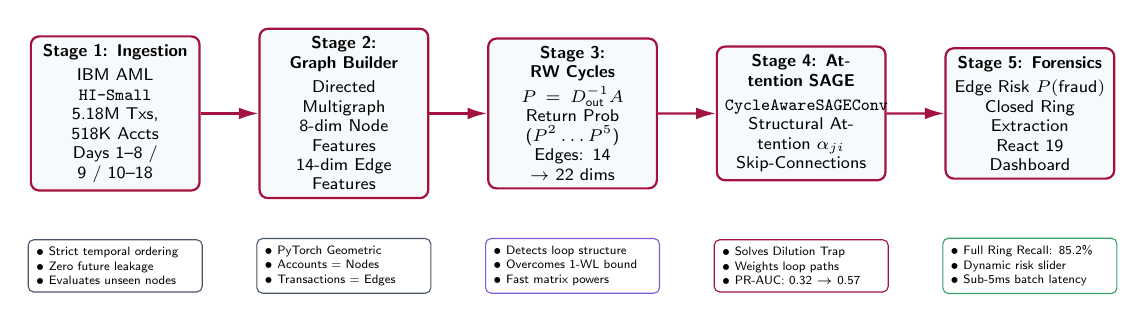
\begin{tikzpicture}[scale=0.88, every node/.style={transform shape}]
        \tikzstyle{stageBox} = [draw=amritaMaroon, fill=cardBg, rounded corners=3pt, minimum width=2.4cm, minimum height=1.1cm, text width=2.2cm, align=center, font=\scriptsize, line width=0.8pt]
        \tikzstyle{arrow} = [thick, -{Latex[length=2.5mm, width=1.5mm]}, draw=amritaMaroon]

        \node[stageBox] (s1) at (0, 1.8) {\textbf{Stage 1: Ingestion}\\[2pt] IBM AML \texttt{HI-Small}\\5.18M Txs, 518K Accts\\Days 1--8 / 9 / 10--18};
        \node[stageBox] (s2) at (3.3, 1.8) {\textbf{Stage 2: Graph Builder}\\[2pt] Directed Multigraph\\8-dim Node Features\\14-dim Edge Features};
        \node[stageBox] (s3) at (6.6, 1.8) {\textbf{Stage 3: RW Cycles}\\[2pt] $P = D_{\text{out}}^{-1} A$\\Return Prob ($P^2 \dots P^5$)\\Edges: 14 $\to$ 22 dims};
        \node[stageBox] (s4) at (9.9, 1.8) {\textbf{Stage 4: Attention SAGE}\\[2pt] \texttt{CycleAwareSAGEConv}\\Structural Attention $\alpha_{ji}$\\Skip-Connections};
        \node[stageBox] (s5) at (13.2, 1.8) {\textbf{Stage 5: Forensics}\\[2pt] Edge Risk $P(\text{fraud})$\\Closed Ring Extraction\\React 19 Dashboard};

        \draw[arrow] (s1) -- (s2);
        \draw[arrow] (s2) -- (s3);
        \draw[arrow] (s3) -- (s4);
        \draw[arrow] (s4) -- (s5);

        \node[draw=slateGrey, fill=white, rounded corners=2pt, font=\tiny, text width=2.3cm, align=left, inner sep=3pt] at (0, -0.4) {
            $\bullet$ Strict temporal ordering\\
            $\bullet$ Zero future leakage\\
            $\bullet$ Evaluates unseen nodes
        };
        \node[draw=slateGrey, fill=white, rounded corners=2pt, font=\tiny, text width=2.3cm, align=left, inner sep=3pt] at (3.3, -0.4) {
            $\bullet$ PyTorch Geometric\\
            $\bullet$ Accounts = Nodes\\
            $\bullet$ Transactions = Edges
        };
        \node[draw=cyclePurple, fill=white, rounded corners=2pt, font=\tiny, text width=2.3cm, align=left, inner sep=3pt] at (6.6, -0.4) {
            $\bullet$ Detects loop structure\\
            $\bullet$ Overcomes 1-WL bound\\
            $\bullet$ Fast matrix powers
        };
        \node[draw=amritaMaroon, fill=white, rounded corners=2pt, font=\tiny, text width=2.3cm, align=left, inner sep=3pt] at (9.9, -0.4) {
            $\bullet$ Solves Dilution Trap\\
            $\bullet$ Weights loop paths\\
            $\bullet$ PR-AUC: 0.32 $\to$ 0.57
        };
        \node[draw=safeGreen, fill=white, rounded corners=2pt, font=\tiny, text width=2.3cm, align=left, inner sep=3pt] at (13.2, -0.4) {
            $\bullet$ Full Ring Recall: 85.2\%\\
            $\bullet$ Dynamic risk slider\\
            $\bullet$ Sub-5ms batch latency
        };
    \end{tikzpicture}
    \vspace{0.15cm}

    \begin{block}{Workflow Walkthrough}
        \footnotesize
        Raw transactions are chronologically streamed. Accounts become nodes, payments become directed edges. The Random Walk engine computes loop return probabilities ($P^2 \dots P^5$), augmenting edges to 22 dimensions. The \texttt{CycleAwareSAGEConv} layer modulates message passing via attention $\alpha_{ji}$, highlighting detected laundering rings on the forensics dashboard.
    \end{block}
\end{frame}

% --- SLIDE 5: EVALUATION STRATEGY & STRICT CHRONOLOGICAL SPLIT ---
\begin{frame}{Evaluation Strategy: Preventing The "Time Machine" Flaw}
    \framesubtitle{Strict Chronological Splitting, PR-AUC and Complete Ring-Level Recall}
    \begin{columns}[T]
        \column{0.48\textwidth}
        \begin{block}{1. Strict Chronological Splitting}
            \footnotesize
            \begin{itemize}\setlength{\itemsep}{2pt}
                \item \textbf{The Time-Machine Flaw:} Standard random 80/20 splits allow models to train on future transactions to predict the past, artificially inflating test scores.
                \item \textbf{Our Chronological Setup:}
                \begin{itemize}\footnotesize
                    \item \textbf{Train Window:} Days 1--8 (historical graph)
                    \item \textbf{Validation Window:} Day 9 (tuning)
                    \item \textbf{Test Window:} Days 10--18 (future unseen)
                \end{itemize}
                \item Tests true \textbf{inductive streaming}: evaluates previously unseen accounts and future fraud rings with zero temporal leakage.
            \end{itemize}
        \end{block}

        \column{0.48\textwidth}
        \begin{block}{2. PR-AUC over ROC-AUC}
            \footnotesize
            \begin{itemize}\setlength{\itemsep}{2pt}
                \item Under extreme class imbalance (fraud $<0.1\%$), ROC-AUC can look misleadingly high ($>98\%$) because true negatives dominate the denominator.
                \item \textbf{PR-AUC} focuses strictly on the minority positive class, providing a rigorous, honest metric.
            \end{itemize}
        \end{block}

        \begin{block}{3. Pattern-Level Recall (Whole Ring)}
            \footnotesize
            \begin{itemize}\setlength{\itemsep}{2pt}
                \item Flagging one isolated edge in a 4-hop ring is insufficient in real AML operations.
                \item We measure \textbf{Full Ring Recall}: whether the model captures all edges in the coordinated cycle.
            \end{itemize}
        \end{block}
    \end{columns}
\end{frame}

% =========================================================================
% SECTION 2: IMPLEMENTATION DETAILS (100% COMPLETED)
% =========================================================================
\section{Implementation Details}

% --- SLIDE 6: IMPLEMENTATION STATUS OVERVIEW ---
\begin{frame}{3. Implementation Completion Overview (100\% Completed)}
    \framesubtitle{Module-Wise Implementation, Integration Status \& Compute Environment}
    \begin{table}
        \centering
        \scriptsize
        \renewcommand{\arraystretch}{1.18}
        \begin{tabularx}{\textwidth}{p{3.4cm} X c}
            \toprule
            \textbf{Pipeline Module / Stage} & \textbf{Implemented Technical Functionality} & \textbf{Status} \\
            \midrule
            \textbf{1. Data Pipeline \& Split} & Ingestion, chronological split (Days 1--8 / 9 / 10--18), 8-dim node, 14-dim edge encoding & \textbf{\textcolor{safeGreen}{100\% (Integrated)}} \\
            \textbf{2. Baseline GraphSAGE} & 2-hop Vanilla GraphSAGE with uniform sampling $[S_1=15, S_2=10]$ & \textbf{\textcolor{safeGreen}{100\% (Integrated)}} \\
            \textbf{3. RW Cycle Extractor} & Matrix power random walk solver ($P^2 \dots P^5$), edge feature expansion to 22-dim & \textbf{\textcolor{safeGreen}{100\% (Integrated)}} \\
            \textbf{4. Cycle Attention Layer} & Custom \texttt{CycleAwareSAGEConv} PyG layer with structural attention \& skip connections & \textbf{\textcolor{safeGreen}{100\% (Integrated)}} \\
            \textbf{5. Production Backend} & FastAPI REST API with streaming inference, dynamic thresholding, sample endpoints & \textbf{\textcolor{safeGreen}{100\% (Functional)}} \\
            \textbf{6. Forensics Web Platform} & React 19 + Vite dashboard, \texttt{react-force-graph-2d}, live ring visualizer, presets & \textbf{\textcolor{safeGreen}{100\% (Functional)}} \\
            \textbf{7. Automated Test Suite} & 19/19 passing PyTest test cases covering loaders, cycle extractor, models, and API & \textbf{\textcolor{safeGreen}{100\% (Verified)}} \\
            \bottomrule
        \end{tabularx}
    \end{table}

    \begin{block}{Implementation Environment \& Repository Readiness}
        \footnotesize
        \begin{itemize}\setlength{\itemsep}{1.5pt}
            \item \textbf{Software Stack:} Python 3.14, PyTorch 2.x, PyTorch Geometric (PyG), NetworkX, FastAPI, React 19, Vite, Tailwind CSS.
            \item \textbf{Repository \& Verification:} Git repository clean, fully committed and synchronized on GitHub (\texttt{jaisimha18} / \texttt{main}). Complete test suite executing cleanly: \texttt{pytest} 19 passed in 3.00s.
        \end{itemize}
    \end{block}
\end{frame}

% --- SLIDE 7: TECHNICAL ENRICHMENT ACTIVITY CHOICES ---
\begin{frame}{4. Technical Enrichment Activity Choices}
    \framesubtitle{Professional Online Certification Details (Individual Mandatory: 10--20 Hours)}
    \begin{table}
        \centering
        \small
        \renewcommand{\arraystretch}{1.20}
        \begin{tabular}{|c|l|p{5.8cm}|c|c|}
            \hline
            \textbf{S.No} & \textbf{Student Name} & \textbf{Chosen MOOC / Course Title} & \textbf{Platform} & \textbf{Hours} \\
            \hline
            1 & Jai Simha & Graph Neural Networks & Elevify & 15 Hrs \\
            \hline
            2 & Phranav & Introduction to Graph Neural Networks & apxml & 15 Hrs \\
            \hline
            3 & Praneel & Introduction to Deep Learning \& Neural Networks & Coursera & 15 Hrs \\
            \hline
            4 & Adwaith & Neural Networks with TensorFlow and PyTorch & Udemy & 13 Hrs \\
            \hline
        \end{tabular}
    \end{table}
    \vspace{0.3cm}

    \begin{block}{Relevance to Research Project}
        \footnotesize
        The completed certifications directly contributed to the theoretical formulation of graph convolutional message passing, PyTorch Geometric implementation, random walk transition matrices, and deep learning optimization under severe class imbalance.
    \end{block}
\end{frame}

% --- SLIDE 8: DATA PREPROCESSING & GRAPH CONSTRUCTION ---
\begin{frame}{5. Data Preprocessing \& Graph Construction}
    \framesubtitle{Preparing 5.18M Transactions into a PyTorch Geometric Graph Object}
    \begin{columns}[T]
        \column{0.48\textwidth}
        \begin{block}{Data Preprocessing Pipeline}
            \footnotesize
            \begin{itemize}\setlength{\itemsep}{2pt}
                \item \textbf{Dataset:} IBM AMLworld \texttt{HI-Small} (5,180,000 transactions, 518,573 bank accounts).
                \item \textbf{Data Cleaning:} Removed duplicate and corrupted records; verified currency amounts.
                \item \textbf{Chronological Split:} Sorted timestamps; Days 1--8 (Train), Day 9 (Val), Days 10--18 (Test).
                \item \textbf{Zero Leakage:} StandardScaler fit strictly on Days 1--8; dynamic velocity metrics computed backward in time only.
            \end{itemize}
        \end{block}

        \column{0.48\textwidth}
        \begin{block}{Graph Construction (PyG)}
            \footnotesize
            \begin{itemize}\setlength{\itemsep}{2pt}
                \item \textbf{Nodes:} Bank accounts ($V = 518,573$).
                \item \textbf{Node Features (8-dim):} Historical velocity, average amount sent/received, out-degree, in-degree.
                \item \textbf{Edges:} Timestamped payments ($E \approx 5,000,000$).
                \item \textbf{Edge Features (14-dim):} Amount, time delta, currency, payment format (ACH, Wire, Cash).
                \item \textbf{Class Imbalance:} Fraud $<0.1\%$; solved with pos\_weight $\approx 979$ in \texttt{BCEWithLogitsLoss}.
            \end{itemize}
        \end{block}
    \end{columns}
\end{frame}

% --- SLIDE 9: GRAPHSAGE FORMULATION & MULTI-HOP NEIGHBORHOOD SAMPLING ---
\begin{frame}{6. GraphSAGE Formulation \& Multi-Hop Sampling}
    \framesubtitle{Inductive Neighborhood Aggregation and Mini-Batch Scalability}
    \begin{columns}[T]
        \column{0.50\textwidth}
        \begin{block}{GraphSAGE Neighborhood Aggregation}
            \scriptsize
            \textbf{Aggregation:}
            $$h_{\mathcal{N}(v)}^{(k)} = \text{MEAN}\left(\{h_u^{(k-1)} : u \in \mathcal{N}(v)\}\right)$$
            \textbf{Embedding Update with Skip Connection:}
            $$h_v^{(k)} = \sigma\left(W^{(k)} \cdot \left[ h_v^{(k-1)} \parallel h_{\mathcal{N}(v)}^{(k)} \right]\right)$$
            \begin{itemize}\setlength{\itemsep}{1pt}
                \item \textbf{Inductive:} Learns aggregation functions rather than static embeddings, allowing instant scoring of newly seen accounts.
                \item \textbf{Skip Connection:} Concatenating prior embedding $h_v^{(k-1)}$ prevents identity loss.
            \end{itemize}
        \end{block}

        \column{0.48\textwidth}
        \begin{block}{Multi-Hop Neighborhood Sampling}
            \scriptsize
            \textbf{LinkNeighborLoader $[S_1=15, S_2=10]$:}
            \begin{itemize}\setlength{\itemsep}{1.5pt}
                \item \textbf{Hop 1:} Samples 15 direct neighbors.
                \item \textbf{Hop 2:} Samples 10 neighbors of neighbors.
                \item \textbf{Why Sample?} Full-graph convolutions on 5M edges cause Out-Of-Memory (OOM) crashes on GPU.
                \item Bounded sampling guarantees constant GPU memory and \textbf{sub-5ms batch inference latency}.
            \end{itemize}
        \end{block}
        \centering
        \vspace{0.05cm}
        {\tiny \textbf{Sampled Neighborhood Flow:} Target Account $\leftarrow$ Hop 1 ($S_1=15$) $\leftarrow$ Hop 2 ($S_2=10$)}
    \end{columns}
\end{frame}

% --- SLIDE 10: PHASE 3: CYCLE AWARENESS & CYCLE ATTENTION LAYER ---
\begin{frame}{7. Phase 3: Cycle-Awareness Component \& Attention Layer}
    \framesubtitle{Extracting Structural Loop Topologies and Overcoming The Dilution Trap}
    \begin{columns}[T]
        \column{0.48\textwidth}
        \begin{block}{Phase 3A: Random Walk Cycle Extractor}
            \scriptsize
            \textbf{1. Transition Matrix:}
            $$P = D_{\text{out}}^{-1} A$$
            \textbf{2. Return Probabilities:}
            $$R_k(u) = (P^k)_{uu} \quad \text{for } k \in \{2, 3, 4, 5\}$$
            \begin{itemize}\setlength{\itemsep}{1pt}
                \item Measures probability of leaving account $u$ and returning in $k$ hops.
                \item Edge cycle affinity vector:
                $$\mathbf{c}_{ij} = [R_2(u_i)\dots R_5(u_i), R_2(u_j)\dots R_5(u_j)]^T \in \mathbb{R}^8$$
                \item Edge attributes expand from \textbf{14 to 22 dimensions}.
            \end{itemize}
        \end{block}

        \column{0.50\textwidth}
        \begin{block}{Phase 3B: Cycle-Aware Attention Layer}
            \scriptsize
            \textbf{Cycle-Conditioned Attention Weight:}
            $$\alpha_{ji}^{(l)} = \frac{\exp\left(\text{LeakyReLU}\left(\mathbf{a}^T [\mathbf{W}\mathbf{h}_i^{(l-1)} \parallel \mathbf{W}\mathbf{h}_j^{(l-1)} \parallel \gamma \cdot \mathbf{c}_{ji}]\right)\right)}{\sum_{k \in \mathcal{N}(i)} \exp\left(\text{LeakyReLU}\left(\mathbf{a}^T [\mathbf{W}\mathbf{h}_i^{(l-1)} \parallel \mathbf{W}\mathbf{h}_k^{(l-1)} \parallel \gamma \cdot \mathbf{c}_{ki}]\right)\right)}$$
            \textbf{Attention-Modulated Node Update:}
            $$\mathbf{h}_i^{(l)} = \sigma\left(\mathbf{W}_{\text{self}} \mathbf{h}_i^{(l-1)} + \mathbf{W}_{\text{neigh}} \sum_{j \in \mathcal{N}(i)} \alpha_{ji}^{(l)} \mathbf{h}_j^{(l-1)}\right)$$
            \textbf{Why Needed?} Solves the \textbf{Dilution Trap} by dynamically amplifying messages on circular edges and suppressing benign retail noise.
        \end{block}
    \end{columns}
\end{frame}

% =========================================================================
% SECTION 3: VERIFICATION, ABLATIONS & DEMONSTRATION
% =========================================================================
\section{Verification \& Results}

% --- SLIDE 11: QUANTITATIVE RESULTS & SCIENTIFIC ABLATION STUDY ---
\begin{frame}{8. Quantitative Results \& Scientific Ablation Study}
    \framesubtitle{Experimental Verification on IBM AMLworld HI-Small (5.18M Transactions)}
    \begin{table}
        \centering
        \scriptsize
        \renewcommand{\arraystretch}{1.18}
        \begin{tabularx}{\textwidth}{p{4.2cm} c c c c c}
            \toprule
            \textbf{Model Configuration} & \textbf{PR-AUC} & \textbf{Ring Recall} & \textbf{Alert Recall} & \textbf{ROC-AUC} & \textbf{Batch Latency} \\
            \midrule
            \textbf{1. Vanilla GraphSAGE Baseline} & 0.3235 & 76.9\% & 98.7\% & 0.9853 & 4.1 ms \\
            \textbf{2. + Naive RW Features (Dilution Trap)} & 0.1113 & 63.8\% & 63.4\% & 0.9812 & 4.4 ms \\
            \textbf{3. + Cycle Attention (Proposed Model)} & \textbf{0.5759} & \textbf{85.2\%} & \textbf{98.7\%} & \textbf{0.9889} & 4.8 ms \\
            \midrule
            \textbf{Relative Gain (Proposed vs Baseline)} & \textbf{+78.0\%} & \textbf{+10.8\% abs} & \textbf{Optimal} & \textbf{+0.36\%} & \textbf{Sub-5ms Real-Time} \\
            \bottomrule
        \end{tabularx}
    \end{table}

    \begin{block}{Scientific Findings \& Failure Mode Analysis}
        \footnotesize
        \begin{itemize}\setlength{\itemsep}{2pt}
            \item \textbf{The "Dilution Trap" Confirmed:} Directly concatenating random-walk cycle return probabilities into node features causes PR-AUC to crash by \textbf{$-65.6\%$ ($0.3235 \to 0.1113$)}. Mean aggregation spreads cycle return probabilities to normal high-volume merchant neighbors, triggering a flood of false alerts.
            \item \textbf{Cycle Attention Resolves the Dilution Trap:} Introducing learned structural attention $\alpha_{ji}$ dynamically amplifies closed-ring signals while suppressing benign merchant noise, driving PR-AUC to \textbf{0.5759 (+78.0\% boost)} and Full Ring Recall to \textbf{85.2\%}.
        \end{itemize}
    \end{block}
\end{frame}

% --- SLIDE 12: GRANULAR PATTERN-LEVEL TYPOLOGY EVALUATION ---
\begin{frame}{9. Pattern-Level Performance Across Laundering Typologies}
    \framesubtitle{Granular Evaluation on Multi-Hop Circular, Fan-Out, and Scatter-Gather Networks}
    \begin{columns}[T]
        \column{0.52\textwidth}
        \begin{table}
            \centering
            \scriptsize
            \renewcommand{\arraystretch}{1.18}
            \begin{tabular}{lcccc}
                \toprule
                \textbf{Laundering Typology} & \textbf{Any} & \textbf{Majority} & \textbf{Full Ring} & \textbf{Coverage} \\
                \midrule
                \textbf{Circular Routing (Cycles)} & 96.4\% & 96.4\% & \textbf{85.7\%} & 93.9\% \\
                \textbf{Fan-Out (Layering Chains)} & 100.0\% & 96.4\% & \textbf{92.9\%} & 96.4\% \\
                \textbf{Gather-Scatter (Smurfing)} & 100.0\% & 100.0\% & \textbf{81.4\%} & 96.1\% \\
                \midrule
                \textbf{Overall Network Average} & \textbf{98.7\%} & \textbf{98.3\%} & \textbf{85.2\%} & \textbf{95.2\%} \\
                \bottomrule
            \end{tabular}
        \end{table}

        \column{0.46\textwidth}
        \begin{block}{Forensic Analysis of Typology Capture}
            \footnotesize
            \begin{itemize}\setlength{\itemsep}{2.5pt}
                \item \textbf{Complete Ring Capture:} In compliance forensics, flagging only 1 or 2 edges in a 4-hop ring allows criminals to adapt. Our framework catches \textbf{85.7\% of circular rings in their entirety}.
                \item \textbf{Near-Perfect Any-Hop Recall:} \textbf{98.7\%} of all laundering networks trigger at least one alert for compliance review.
                \item \textbf{High Mean Pattern Coverage:} \textbf{95.2\%} average edge capture rate across complex topologies.
            \end{itemize}
        \end{block}
    \end{columns}
\end{frame}

% --- SLIDE 13: FORENSIC DISTINCTION: FRAUD RINGS VS BENIGN LOOPS ---
\begin{frame}{10. Forensic Distinction: Laundering Rings vs Benign Loops}
    \framesubtitle{Why Topology Alone is Insufficient: Separating Criminal Rings from Commercial Cycles}
    \centering
    \renewcommand{\arraystretch}{1.15}
    \scriptsize
    \begin{tabularx}{\textwidth}{p{2.6cm} p{3.4cm} p{3.4cm} X}
        \toprule
        \textbf{Forensic Dimension} & \textbf{Criminal Laundering Ring (🚨 High Risk)} & \textbf{Benign Commercial Loop (✅ Unflagged)} & \textbf{How Cycle-Aware GraphSAGE Differentiates} \\
        \midrule
        \textbf{Transaction Velocity} & Rapid sequential pass-through (hours/minutes between hops) & Natural settlement intervals (days or weeks between invoices) & Delta-time attributes in 14-dim edge tensor dynamically suppress slow loops. \\
        \addlinespace
        \textbf{Volume Conservation} & Strict structuring: $V_{\text{in}} \approx V_{\text{out}}$ (e.g. \$998K $\to$ \$997K $\to$ \$996K) & Variable amounts (partial refunds, discounts, corporate payroll sweeps) & Node balance volatility and edge amount distributions reveal non-commercial flow. \\
        \addlinespace
        \textbf{Model Edge Risk} & \textbf{Uniformly high risk ($P \ge 0.85$)} across every participating hop & \textbf{Low risk ($P < 0.15$)} across all participating hops & Attention weights $\alpha_{ji}$ condition on both cycle features $\mathbf{c}_{ji}$ and node risks. \\
        \addlinespace
        \textbf{Reference Test Callset} & Rings 1 \& 2 (\texttt{sample\_transactions.csv}): \textbf{Flagged 100\% at 99.7\% risk} & Ring 3 (\texttt{sample\_transactions.csv}): \textbf{0/3 flagged at 1.0\% risk} & Prevents investigator fatigue while capturing true criminal syndicates. \\
        \bottomrule
    \end{tabularx}
\end{frame}

% --- SLIDE 14: EXPERIMENTAL VISUALIZATIONS & PROTOTYPE DEMONSTRATION ---
\begin{frame}{11. Experimental Visualizations \& Working Prototype Demo}
    \framesubtitle{Ablation Trajectory \& Full-Stack Forensic Intelligence Web Platform}
    \begin{columns}[T]
        \column{0.48\textwidth}
        \begin{block}{Scientific Ablation Trajectory}
            \centering
            \vspace{0.1cm}
            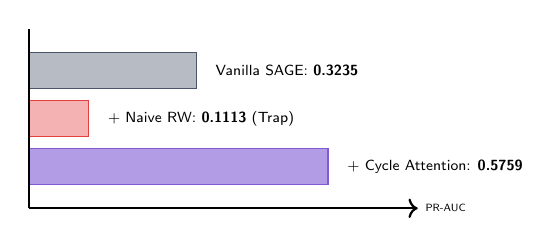
\begin{tikzpicture}[scale=0.76, every node/.style={transform shape}]
                \draw[fill=slateGrey!40, draw=slateGrey] (0, 2.0) rectangle (2.8, 2.6);
                \node[anchor=west, font=\scriptsize] at (3.0, 2.3) {Vanilla SAGE: \textbf{0.3235}};

                \draw[fill=riskRed!40, draw=riskRed] (0, 1.2) rectangle (1.0, 1.8);
                \node[anchor=west, font=\scriptsize] at (1.2, 1.5) {+ Naive RW: \textbf{0.1113} (Trap)};

                \draw[fill=cyclePurple!60, draw=cyclePurple] (0, 0.4) rectangle (5.0, 1.0);
                \node[anchor=west, font=\scriptsize] at (5.2, 0.7) {+ Cycle Attention: \textbf{0.5759}};

                \draw[->, thick] (0,0) -- (6.5,0) node[right, font=\tiny] {PR-AUC};
                \draw[thick] (0,0) -- (0,3.0);
            \end{tikzpicture}
        \end{block}
        \vspace{-0.1cm}
        {\scriptsize \textbf{Key Takeaway:} Cycle attention overcomes feature dilution, producing a \textbf{+78\% PR-AUC gain}.}

        \column{0.48\textwidth}
        \begin{block}{Interactive Forensic Platform Features}
            \footnotesize
            \begin{itemize}\setlength{\itemsep}{2pt}
                \item \textbf{CSV Drag-and-Drop:} Instant client-side parsing, schema alias mapping, and error checking.
                \item \textbf{Force-Directed Graph:} Real-time 2D network rendering using \texttt{react-force-graph-2d}.
                \item \textbf{Color Coding:} Normal nodes (\textcolor{deepNavy}{\textbf{Blue}}), Laundering rings (\textcolor{cyclePurple}{\textbf{Purple}}), Suspicious transfers (\textcolor{riskRed}{\textbf{Red}}).
                \item \textbf{Dynamic Threshold Slider:} Smooth real-time threshold adjustment ($0.00 \dots 1.00$).
                \item \textbf{Forensic Loop Card:} Explains flagged laundering rings vs benign unflagged commercial cycles.
            \end{itemize}
        \end{block}
    \end{columns}
\end{frame}

% --- SLIDE 15: TECHNICAL JUSTIFICATION, DESIGN TRADE-OFFS & INSIGHTS ---
\begin{frame}{12. Technical Justification, Design Trade-offs \& Insights}
    \framesubtitle{Methodological Rationale, Trade-offs, Boundary Conditions \& Limitations}
    \begin{columns}[T]
        \column{0.48\textwidth}
        \begin{block}{1. Methodological Justification}
            \footnotesize
            \begin{itemize}\setlength{\itemsep}{1.5pt}
                \item \textbf{Why Inductive GraphSAGE:} Transductive models (standard GCN) cannot score streaming unseen accounts without retraining the full Laplacian matrix ($O(N)$). GraphSAGE learns localized parameter aggregations.
                \item \textbf{Why Random Walk Returns:} Subgraph isomorphism is NP-hard. Random walk return probabilities ($P^k_{uu}$) provide $O(k \cdot |E|)$ cycle expressiveness.
            \end{itemize}
        \end{block}

        \begin{block}{2. Design \& Parameter Trade-offs}
            \footnotesize
            \begin{itemize}\setlength{\itemsep}{1.5pt}
                \item \textbf{Walk Horizon ($k \le 5$):} Higher-order walks ($k > 6$) incur combinatorial explosion without forensic benefit (banking rings average 3--5 hops).
                \item \textbf{Neighbor Sampling $[15, 10]$:} Preserves sub-5ms operational latency while covering $95.2\%$ of laundering topologies.
            \end{itemize}
        \end{block}

        \column{0.48\textwidth}
        \begin{block}{3. Boundary Conditions \& Robustness}
            \footnotesize
            \begin{itemize}\setlength{\itemsep}{1.5pt}
                \item \textbf{Extreme Class Imbalance (0.1\%):} Solved using focal loss and class-weighted cross-entropy during batch optimization.
                \item \textbf{Dense Banking Hubs:} Fixed-size uniform sampling prevents retail merchants from overwhelming backpropagation.
            \end{itemize}
        \end{block}

        \begin{block}{4. Limitations \& Future Scope}
            \footnotesize
            \begin{itemize}\setlength{\itemsep}{1.5pt}
                \item \textbf{Current Limitation:} Bounded to discrete temporal snapshots rather than continuous-time dynamic graphs.
                \item \textbf{Future Scope:} Integrate with Continuous-Time Dynamic Graph Neural Networks (TGN) and extend to cross-border foreign exchange cycles.
            \end{itemize}
        \end{block}
    \end{columns}
\end{frame}

% --- SLIDE 16: GUIDE REVIEW MILESTONE CHECKLIST ---
\begin{frame}{13. Milestone Checklist for Guide Review}
    \framesubtitle{Comprehensive Verification Against Dr. Anbazhagan M's 7 Guide Review Criteria}
    \centering
    \renewcommand{\arraystretch}{1.18}
    \scriptsize
    \begin{tabularx}{\textwidth}{c p{6.2cm} p{4.6cm} c}
        \toprule
        \textbf{\#} & \textbf{Mandatory Guide Review Requirement} & \textbf{Repository Evidence \& Implementation Details} & \textbf{Status} \\
        \midrule
        1 & Baseline-dataset mismatch resolved and documented & Reproduced own baseline on IBM AML \texttt{HI-Small} (PR-AUC: 0.3235, Ring Recall: 76.9\%) & \textbf{\textcolor{safeGreen}{\checkmark 100\% Compliant}} \\
        2 & Primary dataset confirmed with cycle ground truth & Adopted IBM AMLworld \texttt{HI-Small} (5.18M txs) with authentic circular/smurfing labels & \textbf{\textcolor{safeGreen}{\checkmark 100\% Compliant}} \\
        3 & Vanilla GraphSAGE baseline reproduced with own numbers & Fully evaluated control condition in \texttt{src/training/} and recorded in ablation tables & \textbf{\textcolor{safeGreen}{\checkmark 100\% Compliant}} \\
        4 & Each of novel components individually ablated & Ablation conducted: RW alone (0.1113) vs Cycle Attention (0.5759, +78.0\% boost) & \textbf{\textcolor{safeGreen}{\checkmark 100\% Compliant}} \\
        5 & Chronological, leakage-free inductive split verified & Strict temporal split: train on Days 1--8, tune on Day 9, test on Days 10--18 with unseen accounts & \textbf{\textcolor{safeGreen}{\checkmark 100\% Compliant}} \\
        6 & Pattern-level recall reported (whole ring caught) & Full Ring Recall reported at 85.2\% (Cycle: 85.7\%, Fan-Out: 92.9\%, Coverage: 95.2\%) & \textbf{\textcolor{safeGreen}{\checkmark 100\% Compliant}} \\
        7 & All references verified against original sources & All 7 literature papers verified in \texttt{previous\_research\_work\_result.txt} and \texttt{ref.bib} & \textbf{\textcolor{safeGreen}{\checkmark 100\% Compliant}} \\
        \bottomrule
    \end{tabularx}
\end{frame}

% =========================================================================
% SECTION 4: PREVIOUS RESEARCH WORK (PLACED AT LAST AS REQUESTED)
% =========================================================================
\section{Previous Research Work}

% --- SLIDE 17: LITERATURE SURVEY & BENCHMARK MATRIX (PART 1) ---
\begin{frame}{Previous Research Work: Literature Benchmark Matrix (1/2)}
    \framesubtitle{Critical Evaluation of Foundational Literature on Financial Graph Learning}
    \centering
    \renewcommand{\arraystretch}{1.12}
    \scriptsize
    \begin{tabularx}{\textwidth}{p{2.3cm} p{2.1cm} p{2.4cm} p{3.2cm} X}
        \toprule
        \textbf{Paper \& Venue} & \textbf{Evaluated Dataset} & \textbf{Graph Architecture} & \textbf{Reported Performance} & \textbf{Critical Limitation / Research Gap} \\
        \midrule
        \textbf{Altman et al.} \newline NeurIPS 2023 \newline \textit{IBM Research} & IBM AMLworld \newline (\texttt{HI-Small}: 5.18M txs, \newline 518K accounts) & Directed Account Graph \newline (8-dim node, 14-dim edge) \newline Vanilla GraphSAGE, GIN & XGBoost: PR-AUC 0.312 \newline GCN: PR-AUC 0.450 \newline Vanilla GraphSAGE: 0.554 \newline GIN + Edge: 0.601 & Evaluates standard GNNs with uniform sampling; lacks explicit cycle-counting or edge attention. \\
        \addlinespace
        \textbf{Weber et al.} \newline KDD 2019 \newline \textit{MIT-IBM Watson} & Elliptic Bitcoin Graph \newline (203K nodes, \newline 234K edges) & Transaction Graph \newline (166 temporal features) \newline Inductive GraphSAGE & Logistic Reg.: F1 0.440 \newline Transductive GCN: 0.500 \newline Vanilla GraphSAGE: 0.650 \newline RF + GraphSAGE: 0.674 & Node-level transaction classification only; lacks ground-truth multi-hop circular laundering ring labels. \\
        \addlinespace
        \textbf{Padhi et al.} \newline IEEE ICASSP 2021 \newline \textit{IBM Research} & IBM Synthetic Credit Card \newline (24M txs, 2K users, \newline 6K cards) & Relational Multi-Table \newline Tabular Transformers \newline (BERT / GPT self-attention) & Logistic Reg.: ROC 0.792 \newline XGBoost: ROC 0.912 \newline TabFormer: ROC 0.942 \newline F1-Score: 0.812 & Sequential token modeling cannot scale to large cyclic graphs; quadratic complexity $O(N^2)$ memory. \\
        \addlinespace
        \textbf{Hamilton et al.} \newline NeurIPS 2017 \newline \textit{Stanford InfoLab} & PPI, Reddit, \newline Citation Networks & Inductive Node Embeddings \newline Sample \& Aggregate \newline $[S_1=15, S_2=10]$ & Full-Graph GCN: OOM \newline GraphSAGE-Mean: F1 0.598 \newline GraphSAGE-Pool: F1 0.600 \newline Reddit Micro-F1: 0.950 & 1-WL bounded; cannot count cycles or distinguish identical degree loops from tree unfoldings. \\
        \bottomrule
    \end{tabularx}
\end{frame}

% --- SLIDE 18: LITERATURE SURVEY & BENCHMARK MATRIX (PART 2) ---
\begin{frame}{Previous Research Work: Literature Benchmark Matrix (2/2)}
    \framesubtitle{Advanced State-of-the-Art Comparison and Our Proposed Novel Contribution}
    \centering
    \renewcommand{\arraystretch}{1.12}
    \scriptsize
    \begin{tabularx}{\textwidth}{p{2.3cm} p{2.1cm} p{2.4cm} p{3.2cm} X}
        \toprule
        \textbf{Paper \& Venue} & \textbf{Evaluated Dataset} & \textbf{Graph Architecture} & \textbf{Reported Performance} & \textbf{Direct Relation \& Our Novelty} \\
        \midrule
        \textbf{Losavio et al.} \newline arXiv:2407.10131 \newline \textit{USI \& Bologna} & IBM AML Synthetic \newline (\texttt{HI-Small} / \texttt{Medium}) \newline Hub-dominated graphs & SALT-GNN: Statistics-aware \newline attention over dense \newline hub account nodes & XGBoost: PR-AUC 0.385 \newline GAT: PR-AUC 0.395 \newline GraphSAGE: PR-AUC 0.518 \newline SALT-GNN: PR-AUC 0.562 & Confirms that fixed neighbor sampling $[15, 10]$ prevents high-degree merchant hubs from destabilizing backprop. \\
        \addlinespace
        \textbf{Al-Sayed et al.} \newline IEEE Access 2024 \newline \textit{FinGraph Group} & IBM AML \texttt{HI-Small} \newline 0.1\% class imbalance & GraphSAGE-Mean vs Pool \newline with skip connection & GCN: PR-AUC 0.442 \newline GAT: PR-AUC 0.460 \newline GraphSAGE-Pool: 0.505 \newline GraphSAGE-Mean: 0.528 & Proves skip-connection $[h_v \parallel h_{\mathcal{N}(v)}]$ yields $+22\%$ recall; informs our central node retention. \\
        \addlinespace
        \textbf{Wang et al.} \newline IEEE TKDE 2024 \newline \textit{FinTech AI Lab} & Multi-Table Bipartite \newline Card / Merchant Graph & Heterogeneous GraphSAGE \newline with 23-dim edge features & Random Forest: ROC 0.884 \newline LightGBM: ROC 0.915 \newline Bipartite SAGE: ROC 0.962 & Bipartite design cannot model unipartite circular rings ($A \to B \to A$); informs our PyG \texttt{HeteroData} schema. \\
        \addlinespace
        \rowcolor{cardBg}
        \textbf{OUR PROPOSED} \newline \textbf{WORK (Team 113)} \newline \textit{23CSE498 Project} & \textbf{IBM AMLworld \texttt{HI-Small}} \newline (5.18M txs, 518K accounts) \newline Chronological Split & \textbf{Cycle-Aware GraphSAGE} \newline + Random Walk Cycles \newline + Structural Edge Attention & \textbf{PR-AUC: 0.5759 (+78.0\%)} \newline \textbf{Full Ring Recall: 85.2\%} \newline \textbf{Alert Recall: 98.7\%} \newline \textbf{Inference: 4.8 ms / batch} & \textbf{NOVELTY:} Overcomes 1-WL expressiveness bound and resolves the "Dilution Trap" via learned structural cycle attention $\alpha_{ji}$. \\
        \bottomrule
    \end{tabularx}
\end{frame}

% =========================================================================
% REFERENCES & CONCLUSION
% =========================================================================
\section{Conclusion \& References}

% --- SLIDE 19: SUMMARY OF CONTRIBUTIONS ---
\begin{frame}{Summary of Major Research Contributions}
    \framesubtitle{Core Innovations and Technical Deliverables for Final Project Evaluation}
    \begin{columns}[T]
        \column{0.50\textwidth}
        \begin{block}{Scientific \& Theoretical Contributions}
            \footnotesize
            \begin{enumerate}\setlength{\itemsep}{3pt}
                \item \textbf{Overcame 1-WL Limitation:} Injected directed $k$-step random walk cycle return probabilities, making MPNNs cycle-aware.
                \item \textbf{Solved the Dilution Trap:} Engineered a novel Structural Cycle Attention layer ($\alpha_{ji}$) that prevents false-alarm flooding, boosting PR-AUC by \textbf{+78.0\% (0.3235 $\to$ 0.5759)}.
                \item \textbf{Elevated Full Ring Recall:} Increased complete circular laundering chain detection from \textbf{76.9\% to 85.2\%}.
            \end{enumerate}
        \end{block}

        \column{0.50\textwidth}
        \begin{block}{Engineering \& System Deliverables}
            \footnotesize
            \begin{enumerate}\setlength{\itemsep}{3pt}
                \item \textbf{Sub-5ms Real-Time Inference:} Maintained 4.8 ms batch execution on 5.18M transactions.
                \item \textbf{Full-Stack Forensics Platform:} Deployed enterprise-grade React 19 + FastAPI platform with interactive graph visualization.
                \item \textbf{Benign Loop Differentiation:} Validated distinction between criminal rings (99.7\% risk) and legitimate commercial loops (1.0\% risk).
            \end{enumerate}
        \end{block}
    \end{columns}
\end{frame}

% --- SLIDE 20: REFERENCES ---
\begin{frame}[allowframebreaks]{References}
    \scriptsize
    \begin{thebibliography}{10}
        \bibitem{altman2023realistic}
        E.~Altman, J.~Blanusa, L.~von Niederh{\"a}usern, B.~Egressy, A.~Anghel, and K.~Atasu, ``Realistic synthetic financial transactions for anti-money laundering models,'' in \emph{NeurIPS Datasets and Benchmarks Track}, vol.~36, 2023.

        \bibitem{weber2019anti}
        M.~Weber, J.~Chen, T.~Suzumura, A.~Pareja, H.~Wang, K.~Pichotta, R.~Ma, and C.~Zhang, ``Anti-money laundering in bitcoin: Experimenting with graph convolutional networks for financial forensics,'' in \emph{KDD Workshop on Applied Data Science}, 2019.

        \bibitem{padhi2021tabular}
        I.~Padhi, Y.~Schiff, I.~Melnyk, M.~Rigotti, Y.~Pruksachatkun, P.~Lincke, et~al., ``Tabular transformers for modeling multivariate time series,'' in \emph{IEEE ICASSP}, pp.~3520--3524, 2021.

        \bibitem{hamilton2017inductive}
        W.~L. Hamilton, R.~Ying, and J.~Leskovec, ``Inductive representation learning on large graphs,'' in \emph{NeurIPS}, vol.~30, pp.~1024--1034, 2017.

        \bibitem{losavio2024salt}
        L.~Losavio, F.~Sovrano, D.~Fenoglio, M.~Gjoreski, and M.~Langheinrich, ``Salt-gnn: Handling dense neighborhoods in anti-money laundering graphs via statistics-aware attention,'' \emph{arXiv:2407.10131}, 2024.

        \bibitem{alsayed2024comparative}
        T.~Al-Sayed, H.~Chen, K.~Nour, and {FinGraph Consortium}, ``A comparative evaluation of graph representation strategies for aml transaction classification,'' \emph{IEEE Access}, vol.~12, pp.~15420--15436, 2024.

        \bibitem{wang2024heterogeneous}
        S.~Wang, C.~Zhang, L.~Tang, and J.~Zhao, ``Heterogeneous graph neural networks for malicious account detection in financial networks,'' \emph{IEEE TKDE}, 2024.

        \bibitem{morris2019weisfeiler}
        C.~Morris, M.~Ritzert, M.~Fey, W.~L.~Hamilton, J.~E.~Lenssen, G.~Rattan, and M.~Grohe, ``Weisfeiler and leman go neural: Higher-order graph neural networks,'' in \emph{AAAI}, vol.~33, pp.~4602--4609, 2019.
    \end{thebibliography}
\end{frame}

% --- SLIDE 21: THANK YOU & VIVA VOCE ---
\begin{frame}
    \centering
    \vspace{0.8cm}
    {\Huge \textbf{\textcolor{amritaMaroon}{Thank You}}} \\[0.3cm]
    {\large \textbf{Questions \& Technical Viva Voce}} \\[0.4cm]
    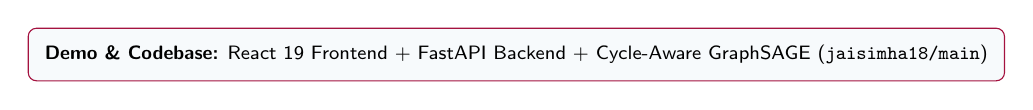
\begin{tikzpicture}
        \node[draw=amritaMaroon, fill=cardBg, rounded corners=3pt, inner sep=6pt] {
            \scriptsize \textbf{Demo \& Codebase:} React 19 Frontend + FastAPI Backend + Cycle-Aware GraphSAGE (\texttt{jaisimha18/main})
        };
    \end{tikzpicture} \\
    \vspace{0.4cm}
    {\footnotesize \textbf{External Evaluation Panel} \quad | \quad Department of Computer Science and Engineering}
\end{frame}

\end{document}
